\documentclass[11pt, oneside]{article}   	% use "amsart" instead of "article" for AMSLaTeX format
\usepackage{geometry}                		% See geometry.pdf to learn the layout options. There are lots.
\geometry{letterpaper}                   		% ... or a4paper or a5paper or ... 
%\geometry{landscape}                		% Activate for for rotated page geometry
%\usepackage[parfill]{parskip}    		% Activate to begin paragraphs with an empty line rather than an indent
\usepackage{graphicx}				% Use pdf, png, jpg, or eps� with pdflatex; use eps in DVI mode
								% TeX will automatically convert eps --> pdf in pdflatex		
\usepackage{amssymb}
\usepackage{amsmath}
\usepackage{parskip}
\usepackage{color}

\title{Dot Product}
%\author{The Author}
%\section{}
% \subsection*{R code}
\date{}							% Activate to display a given date or no date

\graphicspath{{/Users/telliott_admin/Dropbox/Tex/png/}}

% \begin{center} 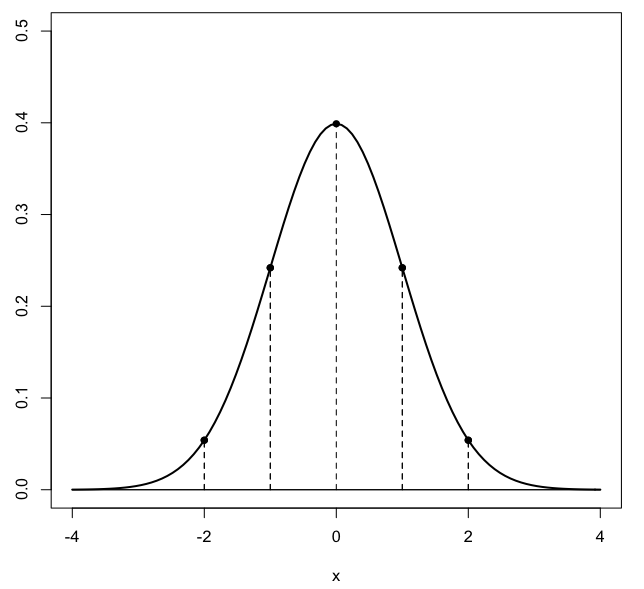
\includegraphics [scale=0.4] {gauss3.png} \end{center}
% \begin{bmatrix} a  &  b \\ c  &  d \end{bmatrix}
% \bigg |_

\begin{document}
\maketitle
\Large
This short write-up introduces a way of multiplying two vectors, the \emph{dot product}, and derives the relationship between the dot product of two vectors and the angle between them.  Suppose we have two vectors
\[ \mathbf{a} = \ \langle a_1,a_2 \rangle \]
\[ \mathbf{b} = \ \langle b_1,b_2 \rangle \]
Geometrically, we might think of these as being one vector extending from the origin in the $x,y$-plane to the point $(a_1,a_2)$, and the other vector extending from the origin to $(b_1,b_2)$.  The dot product is defined as 
\[ \mathbf{a} \cdot \mathbf{b} = a_1 b_1 + a_2 b_2 \]
We can extend this to a pair of vectors in $n$-dimensional space
\[ \mathbf{a} = \ \langle a_1,a_2, \dots a_n \rangle \]
\[ \mathbf{b} = \ \langle b_1,b_2, \dots b_n \rangle \]
\[ \mathbf{a} \cdot \mathbf{b} = a_1 b_1 + a_2 b_2 + \dots + a_n b_n \]
Notice that the two vectors being multiplied (whose dot product is computed) must have the same dimension, the same $n$.  Also, the result of the multiplication---the dot product---is a number.  This is in contrast to another form of vector multiplication (the cross-product) which yields a vector as the result.
\subsection*{Some properties}
The dot product obeys the usual rules:  it is associative, commutative and distributive.  As one example, suppose
\[ \mathbf{b} = \mathbf{c} + \mathbf{d} \]
Then 
\[  \mathbf{a} \cdot \mathbf{b} =  \mathbf{a} \cdot ( \mathbf{c} + \mathbf{d}) = \mathbf{a} \cdot \mathbf{c} + \mathbf{a} \cdot \mathbf{d} \]
You can easily verify this by computing each term of the respective products.
\[ \mathbf{b} = \ \langle b_1,b_2 \rangle \ = \mathbf{c} + \mathbf{d} = \ \langle c_1+d_1,c_2+d_2 \rangle \ \]  
\[  \mathbf{a} \cdot \mathbf{b} = \ \langle a_1(c_1+d_1),a_2(c_2+d_2) \rangle \ \]  
\[ =  \ \langle a_1 c_1+a_1 d_1, a_2 c_2+ a_2 d_2 \rangle \ \]
\[ =  \ \langle a_1 c_1,a_2 c_2> \ + \ \langle a_1 d_1 , a_2 d_2 \rangle \ \]
\[ = \mathbf{a} \cdot \mathbf{c} + \mathbf{a} \cdot \mathbf{d} \]
A second example that we will need below is
\[ ( \mathbf{a} -  \mathbf{b}) \cdot ( \mathbf{a} -  \mathbf{b}) =  \mathbf{a} \cdot \mathbf{a} -  \mathbf{a} \cdot \mathbf{b} -  \mathbf{b} \cdot \mathbf{a} +  \mathbf{b} \cdot \mathbf{b}   \]
Since $\mathbf{a} \cdot \mathbf{b}  = \mathbf{b} \cdot \mathbf{a}$ we have
\[ ( \mathbf{a} -  \mathbf{b}) \cdot ( \mathbf{a} -  \mathbf{b}) =  \mathbf{a} \cdot \mathbf{a} +  \mathbf{b} \cdot \mathbf{b}  - 2 \ \mathbf{a} \cdot \mathbf{b}  \]

\subsection*{Length of a vector}
Recall that the length of a vector $\mathbf{a} = \ \langle a_1,a_2 \rangle $, designated $|\mathbf{a}|$, is computed by a straightforward application of the Pythagorean Theorem:
\[ |\mathbf{a}|^2 = a_1^2 + a_2^2 \]
We leave the result as the square for simplicity.  This is easily extended to more dimensions by sequential application of the same method.  In $\mathbb{R}^3$:
\[ |\mathbf{a}|^2 = a_1^2 + a_2^2 + a_3^2 \]
In $\mathbb{R}^n$:
\[ |\mathbf{a}|^2 = a_1^2 + a_2^2 + \dots + a_n^2 \]
Notice that
\[ |\mathbf{a}|^2 = \mathbf{a} \cdot \mathbf{a} \]

\subsection*{Relation to $\theta$}
Now we are ready for the main idea.  Suppose we draw two vectors $\mathbf{a}$ and $\mathbf{b}$ in $\mathbb{R}^2$ with their tails at the same point.  Designate the angle between them as $\theta$ and the vector representing the side opposite as $\mathbf{c}$.  
\begin{center} 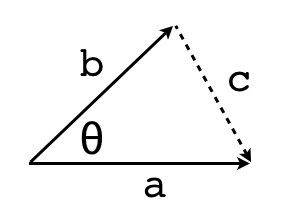
\includegraphics [scale=0.4] {dot1.png} \end{center}
The orientation of  $\mathbf{c}$ doesn't matter for the argument that follows.  As shown
\[ \mathbf{b} + \mathbf{c} = \mathbf{a} \]
\[ \mathbf{c} = \mathbf{a} - \mathbf{b} \]
Compute the dot product of $\mathbf{c}$ with itself
\[ \mathbf{c} \cdot \mathbf{c} = ( \mathbf{a} -  \mathbf{b}) \cdot ( \mathbf{a} -  \mathbf{b}) \]
Recalling the result from above, this is
\[ \mathbf{c} \cdot \mathbf{c} = \mathbf{a} \cdot \mathbf{a} +  \mathbf{b} \cdot \mathbf{b}  - 2 \ \mathbf{a} \cdot \mathbf{b}  \]
Since 
\[ |\mathbf{a}|^2 = \mathbf{a} \cdot \mathbf{a} \]
and so on, we have that
\[ \mathbf{c} \cdot \mathbf{c} =  \mathbf{a} \cdot \mathbf{a} +  \mathbf{b} \cdot \mathbf{b}  - 2 \ \mathbf{a} \cdot \mathbf{b}  \]
\[ |\mathbf{c}|^2 =  |\mathbf{a}|^2 + |\mathbf{b}|^2  - 2  \ \mathbf{a} \cdot \mathbf{b}  \]
Does this remind you of the \emph{Law of Cosines}?  In ordinary trigonometry, we designate the lengths of a triangle's sides as $a,b,c$ and the angle between sides $a$ and $b$ as $\theta$ and the law says that
\[ c^2 = a^2 + b^2 - 2 a b \cos \theta \]
Comparing the two equations, we see that
\[ \mathbf{a} \cdot \mathbf{b} = |\mathbf{a}| \ |\mathbf{b}| \ \cos \theta \]
This relationship is extremely useful because it allows us to compute the cosine of the included angle via the dot product.  Even more important, two vectors which are perpendicular will have $\cos \theta = 0$, so their dot product is zero.  And although we haven't proved it, this result extends to vectors in $\mathbb{R}^n$.
For example, suppose I have the vector
\[ \mathbf{u} = \ \langle p,q \rangle \]
Find a vector $\mathbf{v}$ perpendicular to $\mathbf{u}$.
\[ \mathbf{v} = \ \langle q,-p \rangle \ \]
$\mathbf{v}$ is perpendicular to $\mathbf{u}$ because
\[ \mathbf{u} \cdot \mathbf{v} = p \times q + (- q) \times p = 0 \]
How to find a vector in $\mathbb{R}^5$ perpendicular to $\langle 1,1,1,1,0 \rangle$?
Any vector of the form $\langle 0,0,0,0,k \rangle $ will do, where k is some real number.
\subsection*{Alternate derivation}
Here is another approach which doesn't depend on knowing the law of cosines, but instead requires the rule for subtraction of cosines
\[ \cos (\theta - \phi) = \cos \theta \cos \phi + \sin \theta \sin \phi \]
Go back to the previous figure
\begin{center} 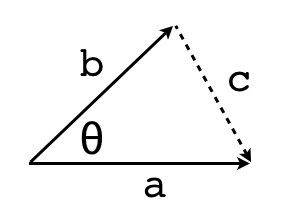
\includegraphics [scale=0.4] {dot1.png} \end{center}
but now imagine that the vector $\mathbf{a}$ forms an angle $\theta_a$ with the $x$-axis and similarly, $\mathbf{b}$ forms an angle $\theta_b$ with the $x$-axis.

If we turn the vector $\mathbf{a}$, then the component of $\mathbf{a}$ that lies along the $x$-axis is $a \cos \theta_a$ (where $a$ is the length of $\mathbf{a}$).  And in a similar vein
\[ a_x = a \cos \theta_a \]
\[ b_x = b \cos \theta_b \]
\[ a_y = a \sin \theta_a \]
\[ b_y = b \sin \theta_b \]
We said that the definition of the dot product is
\[ \mathbf{a} \cdot \mathbf{b} = a_x b_x + a_y b_y \]
\[ = a \cos \theta_a b \cos \theta_b + a \sin \theta_a b \sin \theta_b \]
\[ = ab (\cos \theta_a \cos \theta_b + \sin \theta_a \sin \theta_b) \]
using the subtraction rule this is just
\[ = ab \cos (\theta_a - \theta_b) \]
but since $\theta = \theta_a - \theta_b$
\[ \mathbf{a} \cdot \mathbf{b} = ab \cos \theta \]

\subsection*{Projection}
If $|\mathbf{a}| = 1$ we say that $\mathbf{a}$ is a \emph{unit vector}.  In that case
\[ \mathbf{b} \cdot \mathbf{a} = |\mathbf{b}| \cos \theta \]
Looking at the figure, $|\mathbf{b}| \cos \theta$ is the length of the \emph{projection} of $\mathbf{b}$ on $\mathbf{a}$.  (Recall that the dot product is a scalar---a number---and not a vector).
\begin{center} 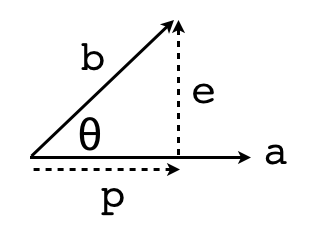
\includegraphics [scale=0.4] {dot3.png} \end{center}
The result, $\mathbf{b} \cdot \mathbf{a} = |\mathbf{b}| \cos \theta$, is the length of the part of $\mathbf{b}$ that extends in the same direction as $\mathbf{a}$.  The corresponding vector is 
\[ \mathbf{p} = (\mathbf{b} \cdot \mathbf{a}) \ \mathbf{a} \]
The other component of $\mathbf{b}$ is the part that is perpendicular to $\mathbf{p}$
\[ \mathbf{p} + \mathbf{e} = \mathbf{b} \]
We compute $\mathbf{e}$ as the difference $\mathbf{b} -  \mathbf{p}$.  $\mathbf{e}$ is the part of $\mathbf{b}$ that is perpendicular to the projection.  As a final note, the formula given here is a simplification for the situation in which $\mathbf{a}$ is a unit vector.  If not, the complete formula is:
\[ \mathbf{p} = \frac{\mathbf{b} \cdot \mathbf{a}}{\mathbf{a} \cdot \mathbf{a}} \ \mathbf{a} \]

\end{document}  